%You can delete all the comments after you have finished your document
%this sets up the defaults for the documents, 12pt font and A4 size. The article type sets this up as such as opposed to letter or memo.

%for the finer points LaTeX see https://en.wikibooks.org/wiki/LaTeX or http://tex.stackexchange.com/

\documentclass[12pt,a4paper]{article}
\usepackage{titlesec} %these are how we import packages, one helps set up footers and title layout
\usepackage{fancyhdr}

% !TEX TS-program = pdflatex
% !TEX encoding = UTF-8 Unicode
\usepackage[utf8]{inputenc} % set input encoding (not needed with XeLaTeX)
\usepackage{graphicx} % support the \includegraphics command and options

% \usepackage[parfill]{parskip} % Activate to begin paragraphs with an empty line rather than an indent

%%% PACKAGES
\usepackage{booktabs} % for much better looking tables
\usepackage{array} % for better arrays (eg matrices) in maths
\usepackage{paralist} % very flexible & customisable lists (eg. enumerate/itemize, etc.)
\usepackage{verbatim} % adds environment for commenting out blocks of text & for better verbatim
\usepackage{subfig} % make it possible to include more than one captioned figure/table in a single float
\usepackage[toc,page]{appendix}
\usepackage{amsthm}
\usepackage[square,sort]{natbib}
\usepackage{tikz}
\usetikzlibrary{er,positioning}
\usepackage{amsmath}
\usepackage{supertabular}
\usepackage{pdfpages}
\usepackage{enumitem}
\usepackage{longtable}
\usepackage{rotating}
\usepackage{pdflscape}
\usepackage{pdfpages}

\graphicspath{{./img/}}

\theoremstyle{definition}
\newtheorem{definition}{Definition}[section]
% These packages are all incorporated in the memoir class to one degree or another...

%header and footer settings
\pagestyle{fancyplain}
\fancyhf{}
\renewcommand{\headrulewidth}{0.5pt}
\renewcommand{\footrulewidth}{0.5pt}
\setlength{\headheight}{15pt}
\fancyhead[L]{Marcin Szczot - 40180425}
\fancyhead[R]{ SOC10101 Honours Project}
\fancyfoot[L]{}
\fancyfoot[C]{\thepage}

%set better section layout
\makeatletter
\renewcommand\subsection{\@startsection {subsection}{1}{2mm} % name, level, indent
                               {3pt plus 2pt minus 1pt} % before skip
                               {3pt plus 0pt} % after skip
                               {\normalfont\bfseries}}
\renewcommand\subsubsection{\@startsection {subsubsection}{2}{4mm} % name, level, indent
                               {3pt plus 2pt minus 1pt} % before skip
                               {3pt plus 0pt} % after skip
                               {\normalfont\bfseries}}
\makeatother
\makeatletter
\renewcommand\section{\@startsection {section}{1}{0mm} % name, level, indent
                               {4pt plus 2pt minus 1pt} % before skip
                               {4pt plus 0pt} % after skip
                               {\bfseries}}
\makeatother


%this starts the document
\begin{document}

%you can import other documents into your main one, these layout the Title and Declarations on its own page.
%you might need to change these to \ if your on Microsoft Windows.
\newcommand{\HRule}{\rule{\linewidth}{0.5mm}}

\begin{titlepage}
	\begin{center}

	\HRule \\[0.4cm]
    	{\Large \bfseries Computing Abstract Argumentation Semantics\par}
	\vspace{0.2cm}
	\HRule \\[1.5cm]

	
    	\vspace{3cm}
	\begin{minipage}{0.4\textwidth}
	\begin{center} \large
        \emph{}\\
        	Marcin Szczot - 40180425
				
   	 \end{center}
    	\end{minipage}
	
	\vspace{2cm}
    	\begin{minipage}{1\textwidth}
    	\begin{center} \large
        
		Submitted in partial fulfilment of \\
		the requirements of Edinburgh Napier University \\
		for the Degree of \\
        	BEng (Hons) Software Engineering
    	\end{center}
    	\end{minipage}

    	\vfill

    	% Bottom of the page
	\begin{minipage}{1\textwidth}
    	\begin{center} \large
		School of Computing
    	\end{center}
    	\end{minipage}
	
	\vspace{1cm}
    	{\large \today}


	\end{center}
\end{titlepage}
%{\large Submitted in partial fulfilment of the requirements of Edinburgh Napier University for the Degree of }

\section*{Authorship Declaration}
\vspace{0.5cm}
\begin{flushleft}
I, (Insert Name eg. Norman Stanley Fletcher), confirm that this dissertation and the work presented in it are my own achievement.\newline

Where I have consulted the published work of others this is always clearly attributed;\newline

Where I have quoted from the work of others the source is always given. With the exception of such quotations this dissertation is entirely my own work;\newline

I have acknowledged all main sources of help; \newline

If my research follows on from previous work or is part of a larger collaborative research project I have made clear exactly what was done by others and what I have contributed myself;\newline

I have read and understand the penalties associated with Academic Misconduct.\newline

I also confirm that I have obtained informed consent from all people I have involved in the work in this dissertation following the School's ethical guidelines.\newline
\end{flushleft}

\begin{flushleft} \large
\emph{Signed:} \\
\end{flushleft}

\vspace{.5cm}

\begin{flushleft} \large
\emph{Date:} \\
\end{flushleft}

\vspace{.5cm}

\begin{flushleft} \large
\emph{Matriculation no: }  \\
\end{flushleft}
\pagebreak

\section*{Data Protection Declaration}
\vspace{0.5cm}
\begin{flushleft}
Under the 1998 Data Protection Act, The University cannot disclose your grade to an unauthorised person. However, other students benefit from studying dissertations that have their grades attached. \newline

\vspace{0.5cm}

Please sign your name below one of the options below to state your preference.\newline
\vspace{0.5cm}

The University may make this dissertation, with indicative grade, available to others.\newline
\vspace{3cm}


The University may make this dissertation available to others, but the grade may not be disclosed.\newline
\vspace{3cm}


The University may not make this dissertation available to others.\newline
\end{flushleft}


\pagebreak

%LaTeX let you define the abstract separately so it wont get sucked into the main document.
\begin{abstract}
\documentclass[../Dissertation.tex]{subfiles}

\begin{document}
	
\end{document}
\end{abstract}
\pagebreak

\tableofcontents % is generated for you
\newpage

\listoftables
%generated in same way as figures
\newpage

\listoffigures
%you may have captions such as equations, listings etc they should all appear as required
%these are done for you as long as you use \begin{figure}[placement settings] .. bla bla ... \end{figure}
\newpage

\section*{Acknowledgements}
Insert acknowledgements here
\subsection*{}
	I would like to thank my cat, dog and family.
\newpage

%-------------------------------------------------------------------------------
% Main content 
%-------------------------------------------------------------------------------
\section{Introduction}
This is my test \cite{dung1995acceptability}

\section{Literature Review}
\subsection{Abstract Argumentation} \label{abstractArgumentation}
Argumentation framework has been introduced by \citet{dung1995} and is central to the theory of abstract argumentation \citep{baroni2011introduction}. It is defined as a pair of a set of arguments, and a binary relation representing the attack relationship between arguments \citep{dung1995}. 

\theoremstyle{definition}
\begin{definition}{Argumentation Framework}
\label{AFdef}\\
An argumentation framework is a pair \textit{AF} = $<$\textit{AR, attacks}$>$ in which \textit{AR} is a set of finite arguments, and \textit{attacks} is a binary relation on \textit{AR}, hence \textit{attacks} $\subseteq$ \textit{AR} $\times$ \textit{AR}, where \textit{AR} $\times$ \textit{AR} = \{(\textit{a}, \textit{b}) $\vert$ \textit{a} $\in$ \textit{AR} and \textit{b} $\in$ \textit{AR}\}
\end{definition}

In definition \ref{AFdef}, \textit{AR} represents a set of arguments and \textit{attacks} represents set of pairs of arguments (\textit{a, b}), where (\textit{a, b}) $\in$ \textit{attacks}. Each pair of arguments in \textit{attacks} represents two arguments being in conflict. Hence, the arguments \textit{a} and \textit{b} from definistion \ref{AFdef} are in conflict and the meaning of \textit{attacks(a, b)} is that \textit{a} attacks \textit{b}. Based on this definition, we can conclude that the set of arguments \textit{AR} is conflict-free if and only if there are no arguments \textit{a} and \textit{b} in \textit{AR} such that \textit{a} attacks \textit{b}, or \textit{b} attacks \textit{a} \citep{dung1995}.

The argumentation framework can be represented as directed graph where the nodes represent abstract arguments and edges the attack relation. This can be seen in figure \ref{fig:argumentationFrameworkFigure}, where argument \textit{a} attacks argument \textit{b}, which in turn attacks argument \textit{c}. \textit{C} is also attacked by argument \textit{d}.
\newpage
\begin{figure}[h]
\tikzset{
    main/.style={draw, rectangle, rounded corners, minimum height=1cm, minimum width=4.5cm},
    arrow/.style={thick,<-,>=stealth}
}
\centering
\begin{tikzpicture}[auto,node distance=1.5cm]
	\node[draw=none,fill=none](a){a};
	\node[draw=none,fill=none][right=of a](b){b};
	\node[draw=none,fill=none][right=of b](c){c};
	\node[draw=none,fill=none][right=of c](d){d};	
  	%%% ARROWS %%%
  	\draw[arrow](b) -- (a);
  	\draw[arrow](c) -- (b);
  	\draw[arrow](c) -- (d);
\end{tikzpicture}
\caption{Argumentation Framework \ref{fig:argumentationFrameworkFigure}}
\label{fig:argumentationFrameworkFigure}
\end{figure}
 
Example of the argumentation framework can also be presented using the following example from \citet{konolige1988defeasible}:
\begin{quote}
Suppose Ralph normally goes fishing on Sundays, but on the Sunday which is
Mother’s day, he typically visits his parents. Furthermore, in the spring of each
leap year, his parents take a vacation, so that they cannot be visited.
\end{quote}
If we assume it is Sunday, Mother's day and a leap year, then three arguments can be formulated from the extract above:
\begin{enumerate}[label=\Alph*]
	\item{Ralph goes fishing because it is Sunday.}
	\item{Ralph does not go fishing because it is Mother's day, hence he visits his parents.}
	\item{Ralph does not go visit his parents, because it is a leap year. Hence, they are on vacation.}
\end{enumerate}
In this example argument \textit{B} attacks argument \textit{A} and argument \textit{C} attacks argument \textit{B}. Since argument \textit{C} can be justified, as it is not attacked, then \textit{B} is defeated and does no longer form a reason against \textit{A}. We can say that argument \textit{C} reinstates argument \textit{A} \citep{caminada2004sake}.


Dung in his paper \citep{dung1995} has also defined notions of \textit{acceptable} and \textit{admissible} arguments, which are as follow:

\begin{definition}{Acceptable argument}
\label{AcceptableArgDef}\\
An argument \textit{a} $\in$ \textit{AR} is said to be \textit{acceptable} with respect to set \textit{S} $\subseteq$ \textit{AR} if and only if for each argument \textit{b} $\in$ \textit{AR} such that (\textit{b}, \textit{a}) $\in$ \textit{attacks}, there are some arguments \textit{c} $\in$ \textit{S} such that (\textit{c}, \textit{b}) $\in$ \textit{attacks}
\end{definition}

Hence it can be said that the argument from given argumentation framework is acceptable with respect to the set only if it is either conflict free, or there exists an argument from the same set that defends given argument. Based on the definition \ref{AcceptableArgDef}, definition of \textit{admissible} set can be concluded:

\begin{definition}{Admissible argument} \label{admissibleArgument}
\label{AdmissibleArgDef}\\
A conflict-free set of arguments \textit{S} is \textit{admissible} if and only if each argument in \textit{S} is acceptable with respect to \textit{S}.
\end{definition}

That means that the set of arguments can be described as admissible only if it is conflict-free and all of its arguments can be defended by other arguments from that set. Both definitions have important role in defining the semantics of abstract argumentation. An argumentation semantics can be described as the formal definition of a method (declarative or procedural) ruling the argument evaluation process \citep{baroni2009semantics}. Hence, they are used to evaluate if the arguments can be justified, by being defended by other arguments in the set, or rejected. 

There are two approaches for defining argumentation semantics: extension and labelling based. In the extension-based approach semantic definition specifies how to derive from an argumentation framework a set of extensions, where an extension \textit{E} of an argumentation framework $<$\textit{AR, attacks}$>$ is simply a subset of \textit{AR}, intuitively representing a set of arguments which can “survive together” or are “collectively acceptable” \citep{baroni2009semantics}. On the other hand labelling-based approach defines how the arguments can be labelled based on the predefined set of labels. Labels define the possible states of argument and those are as follow: 
\begin{itemize}
	\item \textit{in}, when argument can be justified, 
	\item \textit{out} when argument is rejected, and 
	\item \textit{undecided} to any other argument.
\end{itemize}

As shown by Modgil and Caminada, label-based approach is suitable for characterizing argumentation semantics \citep{modgil2009proof}.
\subsection{Argumentation Semantics}
\label{sec:argumentationSemantics}


The original concept of abstract argumentation semantics included complete, stable, preferred and grounded extensions \citep{dung1995}, which was extended by stage \citep{verheij1996two}, ideal \citep{dung2007computing}, and semi-stable \citep{caminada2006semi} semantics. All the sematics are based around the definitions of acceptable and admissible arguments. Definitions of the original semantics as described by \citet{dung1995} are as follow: 

\begin{definition}{Preferred Extension}
\label{def:preferredExtension}\\
A \textit{preferred extension} of an argumentation framework \textit{AF} is a maximal (with respect to set inclusion) admissible set of \textit{AF}.
\end{definition}


From the definition \ref{def:preferredExtension} it can be seen that the preferred extension is the largest set that is able to defend itself from attacks. If we consider example \ref{fig:af1} we can see that the extension \textit{$E_{PR}$} = \{\{a,c\}, \{b\}\}. Argument \textit{c} is attacked by argument \textit{b}, which in turn is defeated by \textit{a}, hence \textit{a} and \textit{c} are preferred extension. Furthermore, \textit{b} is attacked by \textit{a}, but it defends itself. Hence argument \textit{b} is also preferred extension.

\begin{figure}[h]
\tikzset{
    main/.style={draw, rectangle, rounded corners, minimum height=1cm, minimum width=4.5cm},
    arrow/.style={thick,<-,>=stealth}
}
\centering
\begin{tikzpicture}[auto,node distance=1.5cm]
	\node[draw=none,fill=none](c){c};
	\node[draw=none,fill=none][right=of c](b){b};
	\node[draw=none,fill=none][right=of b](a){a};	
  	%%% ARROWS %%%
  	\draw[thick,<-,>=stealth,transform canvas={yshift=0.5em}](b) -- (a);
  	\draw[arrow](c) -- (b);
  	\draw[thick,<-,>=stealth,transform canvas={yshift=-0.2em}](a) -- (b);
\end{tikzpicture}
\caption{Argumentation Framework \ref{fig:af1}}
\label{fig:af1}
\end{figure}

\begin{definition}{Stable Extension}
\label{def:stableExtension}\\
A \textit{conflict-free} set of arguments \textit{S} is called a \textit{stable extension} if and only if \textit{S} attacks each argument which does not belong to \textit{S}.
\end{definition}

Stable extension has more aggressive approach than preferred extension. As in definition \ref{def:stableExtension}, the extension needs to attack all arguments that are not included in it. Based on argumentation framework from example \ref{fig:af1}, the stable extension \textit{$E_{ST}(AF_{\ref{fig:af1}})$} = \{\{a,c\}, \{b\}\}, which is the same as for preferred extension. This is because argument \textit{a} attacks \textit{b}, hence \textit{a} and \textit{c} are included, and argument \textit{b} attack both arguments \textit{a} and \textit{c}. Looking at more complex example in figure \ref{fig:af2}, three stable extensions can be identified as follow \textit{$E_{ST}(AF_{\ref{fig:af2}})$} = \{\{a,c\}, \{a,d\}, \{b,d\}\}.

\begin{figure}[h]
\tikzset{
    main/.style={draw, rectangle, rounded corners, minimum height=1cm, minimum width=4.5cm},
    arrow/.style={thick,<-,>=stealth}
}
\centering
\begin{tikzpicture}[auto,node distance=1.5cm]
	\node[draw=none,fill=none](c){c};
	\node[draw=none,fill=none][left=of c](d){d};
	\node[draw=none,fill=none][right=of c](b){b};
	\node[draw=none,fill=none][right=of b](a){a};	
  	%%% ARROWS %%%
  	\draw[thick,<-,>=stealth,transform canvas={yshift=0.5em}](b) -- (a);
  	\draw[arrow](c) -- (b);
  	\draw[thick,<-,>=stealth,transform canvas={yshift=-0.2em}](a) -- (b);
  	\draw[thick,<-,>=stealth,transform canvas={yshift=-0.2em}](c) -- (d);
  	\draw[thick,<-,>=stealth,transform canvas={yshift=0.5em}](d) -- (c);
\end{tikzpicture}
\caption{Argumentation Framework \ref{fig:af2}}
\label{fig:af2}
\end{figure}

\citet{dung1995} in his paper also defined a skeptical semantics known as grounded extension. This extension is defined in terms of \textit{characteristic function}, which in turn is defined as:

\begin{definition}{Characteristic Function}
\label{def:characteristicFunction}\\
The \textit{characteristic function}, denoted by \textit{F\textsubscript{AF}}, of an argumentation framework \textit{AF} = $<$\textit{AR, attacks}$>$ is defined as follows:
\[F_{AF}:2^{AR} \rightarrow 2^{AR}\]
\[F_{AF}(S)=\{A| \text{A is acceptable with respect to S} \}\]
\end{definition}

\begin{definition}{Grounded Extension}
\label{def:groundedExtension}\\
The \textit{grounded extension} of an argumentation framework \textit{AF}, denoted by \textit{GE\textsubscript{AF}}, is the least fixed point of \textit{F\textsubscript{AF}}.
\end{definition}

Based on the definition of characteristic function and grounded extension it can be noted that the grounded extension has very restrictive approach for its computation, as it only includes the arguments whose defence is "rooted" in initial unattacked argument \citep{baroni2009semantics}. Hence, the grounded extension from figure \ref{fig:af3} is \textit{$E_{GR}(AF_{\ref{fig:af3}})$} = \{\{a,c\}\}. Starting from argument \textit{a}, as it is the only unattacked argument, we reject argument \textit{b} and include \textit{c}. Furthermore, argument \textit{d} is being rejected, as it is attacked by \textit{c}. Although, argument \textit{e} attacks argument \textit{f}, it is attacked by \textit{f} as well. Hence, it cannot be part of grounded extension.

\begin{figure}[h]
\tikzset{
    main/.style={draw, rectangle, rounded corners, minimum height=1cm, minimum width=4.5cm},
    arrow/.style={thick,<-,>=stealth}
}
\centering
\begin{tikzpicture}[auto,node distance=1.5cm]
	\node[draw=none,fill=none](a){a};
	\node[draw=none,fill=none][right=of a](b){b};
	\node[draw=none,fill=none][right=of b](c){c};	
	\node[draw=none,fill=none][right=of c](d){d};
	\node[draw=none,fill=none][right=of d](e){e};
	\node[draw=none,fill=none][right=of e](f){f};			
  	%%% ARROWS %%%
  	\draw[arrow](b) -- (a);
  	\draw[arrow](c) -- (b);
  	\draw[arrow](d) -- (c);
  	\draw[arrow](e) -- (d);
  	\draw[thick,<-,>=stealth,transform canvas={yshift=-0.2em}](e) -- (f);
  	\draw[thick,<-,>=stealth,transform canvas={yshift=0.5em}](f) -- (e);
\end{tikzpicture}
\caption{Argumentation Framework \ref{fig:af3}}
\label{fig:af3}
\end{figure}

\begin{definition}{Complete Extension}
\label{def:completeExtension}\\
An admissible set \textit{S} of arguments is called \textit{complete exension} if and only if each argument which is acceptable with respect to \textit{S}, belongs to \textit{S}.
\end{definition}

Complete extension is defined as a set which is able to defend itself and includes all arguments it defends \citep{baroni2009semantics}. Based on this, we can see that there are three complete extensions in figure \ref{fig:af1}, and those are \textit{$E_{CO}(AF_{\ref{fig:af1}})$} = \{$\emptyset$, \{a,c\}, \{b\}\}. With a more complex argumentation framework in figure \ref{fig:af2}, it can be seen that the complete extension will definitely include empty set, as there are no initial arguments, argument \textit{a}, as it does not defend argument \textit{c} from \textit{d}, and argument \textit{d}, as it only defends itself. Furthermore, \textit{b} attacks \textit{c}, the only attacked of argument \textit{d}, hence set \{b,d\} is a complete extension as well. Additionally, sets \{a,c\} and \{a,d\} are also compltete extensions as both of them are admissible. Hence, the complete extension is \textit{$E_{CO}(AF_{\ref{fig:af2}})$} = \{$\emptyset$, \{a\}, \{d\}, \{a,c\}\, \{a,d\}, \{b,d\}\}.

As mentioned earlier, \citet{dung1995} semantics were further extended with additional semantics. Their definitions are as follow: 

\begin{definition}{Semi-stable Extension}
\label{def:semiStableExtension}\\
Let (\textit{AR}, \textit{attacks}) be an argumentation framework and \textit{Args} $\subseteq$ \textit{AR}. \textit{Args} is called \textit{semi-stable extension} if and only if \textit{Args} is a complete extension where \textit{Args} $\cup$ \textit{$Args^+$} is maximal.
\end{definition}

The idea for semi-stable extension consist in expressing a definite opinion on the largest possible set of arguments, while restricting as much as possible those which are left undecided \citep{baroni2011introduction}, where labelling has been used. Hence, the stable-extension in argumentation framework in figure \ref{fig:af4} is \textit{$E_{SST}(AF_{\ref{fig:af4}})$} = \{\{b,d\}\}, which is also a preferred extension.

\begin{figure}[h]
\tikzset{
    main/.style={draw, rectangle, rounded corners, minimum height=1cm, minimum width=4.5cm},
    arrow/.style={thick,<-,>=stealth}
}
\centering
\begin{tikzpicture}[auto,node distance=1.5cm]
	\node[draw=none,fill=none](a){a};
	\node[draw=none,fill=none][right=of a](b){b};
	\node[draw=none,fill=none][right=of b](c){c};	
	\coordinate[right=0.75cm of c](coordinate);
	\node[draw=none,fill=none][above =0.5cm of coordinate](d){d};
	\node[draw=none,fill=none][below =0.5cm of coordinate](e){e};		
  	%%% ARROWS %%%
  	\draw[thick,<-,>=stealth,transform canvas={yshift=-0.2em}](a) -- (b);
  	\draw[thick,<-,>=stealth,transform canvas={yshift=0.5em}](b) -- (a);
  	\draw[arrow](c) -- (b);
	\draw[thick, -latex] (c.north) to [bend left=45](d.west);
	\draw[thick, -latex] (d.east) to [bend left=90](e.east);
	\draw[thick, -latex] (e.west) to [bend left=45](c.south);
\end{tikzpicture}
\caption{Argumentation Framework \ref{fig:af4}}
\label{fig:af4}
\end{figure}

\begin{definition}{Ideal Extension}
\label{def:idealExtension}\\
The \textit{ideal extension} is the greatest with respect to set inclusion admissible set that is a subset of each preferred extension.
\end{definition}

By its definition the ideal extension satisfies I-maximality and admissibility principles \citep{baroni2009semantics}. The I-maximiality is a property of the set of extensions, without reference to any generic criterion \citep{dunne2006computational}. It is defined as:

\begin{definition}{I-maximality}
\label{def:IMaximality}\\
A set of extensions \textit{E} is I-maximal if and only if $\forall$\textit{$E_1$}, \textit{$E_2$} $\in$ \textit{E}, if \textit{$E_1$} $\subseteq$ \textit{$E_2$} then \textit{$E_1$} = \textit{$E_2$}.
\end{definition}

Perhaps, the ideal semantics can be best explained using the notion of a judgement aggregation context intoduced by \citet{caminada2011judgment}. Given an argumentation framework, if we assume a group of people who all try to accept as much as possible the sets of arguments they all agree on needs to be examined and checked whether this position is still defensible. However, if they are not defensible some of the arguments needs to be abstained from instead of accepting or rejecting them until it becomes defensible. The result is the ideal extension \citep{baroni2011introduction}.

\begin{definition}{Stage Extension}
\label{def:stageExtension}\\
Let (\textit{AR}, \textit{attacks}) be an argumentation framework. A \textit{stage extension} conflict-free set \textit{Args} $\subseteq$ \textit{AR}, where \textit{Args} $\cup$ \textit{$Args^+$} is maximal with respect to set inclusion among all conflict-free sets.
\end{definition}

Stage extension introduced by \citet{verheij1996two} can also be explained in terms of labelling. It is a conflict-free extension where number of arguments labeled \textit{undec} is minimal. 
\newline

\begin{figure}[h]
\tikzset{
    main/.style={draw, rectangle, rounded corners, minimum height=1cm, minimum width=4.5cm},
    arrow/.style={thick,<-,>=stealth}
}
\centering
\begin{tikzpicture}[auto,node distance=1.5cm]
	\node[main](1){Complete Semantics};
	\coordinate[below=of 1](c);
  	\node[main](2)[left=of c]{Grounded Semantics};
  	\node[main](3)[right=of c]{Ideal Semantics};
  	\node[main](4)[below=of c]{Preferred Semantics};
  	\node[main](5)[below=of 4]{Semi-Stable Semantics};
  	\node[main](7)[below=of 5]{Stable Semantics};  	
  	\node[main](6)[right=of 7]{Stage Semantics};
  	%%% ARROWS %%%
  	\draw[arrow](1) -- (2) node[midway] {is a};
  	\draw[arrow](1) -- (3) node[midway] {is a};
  	\draw[arrow](1) -- (4) node[midway] {is a};
  	\draw[arrow](4) -- (5) node[midway] {is a};
  	\draw[arrow](5) -- (7) node[midway] {is a};  	
  	\draw[arrow](6) -- (7) node[midway] {is a};
\end{tikzpicture}
\caption{Relations of semantics}
\label{fig:semanticsRelations}
\end{figure}

Above semantics can be used to decide whether a given argument, or set of arguments can be accepted in terms of set inclusion.  Based on the definitions a number of inclusions between the sets can be conluded. Those are:
\begin{itemize}
	\item{Grounded extension is the smallest complete extension}
	\item{Every preferred extesion is also complete}
	\item{Every stable extension is also semi-stable and stage extension}
\end{itemize}
Furthermore, it can be seen that the complete extension provides the link between preferred extension (credulous semantic), and grounded extension (skeptical smenatics) \citep{dung1995}. It can also be concluded seen that the maximal complete extension is also maximal admissible set. On the other hand the grounded extension is determined by the minimal complete extension \citep{gaggl2009solving}. The relations between the semantics can be seen in figure \ref{fig:semanticsRelations}.


%sceptical and credulous semantics
%sceptical and credulous acceptance of argument
Additional notion of credulous and sceptical semantics has been introduced. Usually, a credulous semantics is intended to capture as much information as possible \citep{dix1995non}, while skeptical makes less committed choices about the justification of the arguments \citep{baroni2007comparing}. As mentioned previosly grounded semantic is a good example of skeptical extension as it always yields exactly one extension, and this extension is admissible \citep{caminada2007comparing}.

Furthermore, argument can be defined as credulous or skeptical in terms of its acceptability. As describe by \citet{arieli2015conflict} an argument \textit{a} $\in$ \textit{Args} is credulously accepted by one type of semantics only if it belongs to some of the semantic extensions of a given argumentation framework. On the other hand, the argument \textit{b} is skeptically accepted by the semantic if it belongs to all of its extensions of a given argumentation framework. This can be represented using argumentation framework \ref{fig:af5}. It has 5 complete extensions: $\emptyset$, {b}, {e}, {b, e}, {a, c, e}, however none of the arguments is skeptically accepted, while \textit{a}, \textit{b}, \textit{c} and \textit{e} are credulously accepted. On the other hand, \{\textit{b, e}\} and \{\textit{a, c, e}\} are preferred, stable, semi-stable and stage extensions of argumentation framework \ref{fig:af5}. It can be seen that only argument \textit{e} is skeptically accepted for all those semantics, while \textit{a}, \textit{b} and \textit{c} are credulously accepted.

\begin{figure}[h]
\tikzset{
    main/.style={draw, rectangle, rounded corners, minimum height=1cm, minimum width=4.5cm},
    arrow/.style={thick,<-,>=stealth}
}
\centering
\begin{tikzpicture}[auto,node distance=1.5cm]
	\node[draw=none,fill=none](a){a};
	\node[draw=none,fill=none][right=of a](b){b};
	\node[draw=none,fill=none][right=of b](c){c};	
	\node[draw=none,fill=none][right=of c](d){d};	
	\coordinate[right=0.75cm of d](coordinate);
	\node[draw=none,fill=none][above =0.5cm of coordinate](e){e};
	\node[draw=none,fill=none][below =0.5cm of coordinate](f){f};		
  	%%% ARROWS %%%
  	\draw[thick,<-,>=stealth,transform canvas={yshift=-0.2em}](a) -- (b);
  	\draw[thick,<-,>=stealth,transform canvas={yshift=0.5em}](b) -- (a);
  	\draw[arrow](c) -- (b);
  	\draw[arrow](d) -- (c);
	\draw[thick, -latex] (d.north) to [bend left=45](e.west);
	\draw[thick, -latex] (e.east) to [bend left=90](f.east);
	\draw[thick, -latex] (f.west) to [bend left=45](d.south);
\end{tikzpicture}
\caption{Argumentation Framework \ref{fig:af5}}
\label{fig:af5}
\end{figure}
\subsection{Approaches to computing argumentation semantics} \label{approaches}

\begin{figure}[h]
	\centering
	\begin{tikzpicture}
	\begin{axis}[
	ybar,
	symbolic x coords={pyglaf, cegartix, argmat-sat, argmat-dvisat, CoQuiAAS, argmat-mpg, goDIAMOND, heureka, conarg, ArgTools, ArgSemSAT, EqArgSolver, argmat-clpb, gg-sts},
	xtick=data,
	x tick label style={rotate=90,anchor=east},
	legend style={at={(0.05,0.1)},anchor=west},
	]
	\addplot table[x=Solver,y=Score]{\completeResults};
	\addplot[draw=red,ultra thick,smooth] table[x=Solver,y=Time]{\completeResults};
	\legend{Score,Time}
	\end{axis}
	\end{tikzpicture}
	\caption{Results of Complete Extension Track from ICCMA 2017}
	\label{fig:coTrack}
\end{figure}

\begin{figure}[h]
	\centering
	\begin{tikzpicture}
	\begin{axis}[
	ybar,
	symbolic x coords={pyglaf,argmat-dvisat,argmat-sat,goDIAMOND,cegartix,ArgTools,argmat-mpg,conarg,CoQuiAAS,gg-sts
	},
	xtick=data,
	x tick label style={rotate=90,anchor=east},
	legend style={at={(0.05,0.1)},anchor=west},
	]
	\addplot table[x=Solver,y=Score]{\idealResults};
	\addplot[draw=red,ultra thick,smooth] table[x=Solver,y=Time]{\idealResults};
	\legend{Score,Time}
	\end{axis}
	\end{tikzpicture}
	
	\caption{Results of Ideal Extension Track from ICCMA 2017}
	\label{fig:idTrack}
	
\end{figure}

\begin{figure}[h]
	\centering
	\begin{tikzpicture}
	\begin{axis}[
	ybar,
	symbolic x coords={pyglaf,goDIAMOND,argmat-sat,cegartix,argmat-mpg,argmat-dvisat,conarg,heureka,ArgSemSAT,ArgTools,EqArgSolver,argmat-clpb,ChimaerArg,CoQuiAAS,gg-sts
	},
	xtick=data,
	x tick label style={rotate=90,anchor=east},
	legend style={at={(0.05,0.1)},anchor=west},
	]
	\addplot table[x=Solver,y=Score]{\stableResults};
	\addplot[draw=red,ultra thick,smooth] table[x=Solver,y=Time]{\stableResults};
	\legend{Score,Time}
	\end{axis}
	\end{tikzpicture}
	
	\caption{Results of Stable Extension Track from ICCMA 2017}
	\label{fig:stTrack}
\end{figure}


\begin{figure}[h]
	\centering
	\begin{tikzpicture}
	\begin{axis}[
	ybar,
	symbolic x coords={argmat-sat,ArgSemSAT,cegartix,pyglaf,goDIAMOND,argmat-mpg,conarg,ArgTools,gg-sts,CoQuiAAS
	},
	xtick=data,
	x tick label style={rotate=90,anchor=east},
	legend style={at={(0.05,0.1)},anchor=west},
	]
	\addplot table[x=Solver,y=Score]{\semiStableResults};
	\addplot[draw=red,ultra thick,smooth] table[x=Solver,y=Time]{\semiStableResults};
	\legend{Score,Time}
	\end{axis}
	\end{tikzpicture}
	
	\caption{Results of Semi Stable Extension Track for ICCMA 2017}
	\label{fig:ssTrack}
\end{figure}


\begin{figure}[h]
	\centering
	\begin{tikzpicture}
	\begin{axis}[
	ybar,
	symbolic x coords={argmat-sat,
		pyglaf,
		cegartix,
		goDIAMOND,
		conarg,
		argmat-mpg,
		ArgTools,
		CoQuiAAS,
		gg-sts,},
	xtick=data,
	x tick label style={rotate=90,anchor=east},
	legend style={at={(0.05,0.1)},anchor=west},
	]
	\addplot table[x=Solver,y=Score]{\stageResults};
	\addplot[draw=red,ultra thick,smooth] table[x=Solver,y=Time]{\stageResults};
	\legend{Score,Time}
	\end{axis}
	\end{tikzpicture}
	
	\caption{Results of Stage Extension Track for ICCMA 2017}
	\label{fig:stgTrack}
\end{figure}



\begin{figure}[h]
	\centering
	\begin{tikzpicture}
	\begin{axis}[
	ybar,
	symbolic x coords={ArgSemSAT,
		argmat-sat,
		pyglaf,
		argmat-dvisat,
		cegartix,
		goDIAMOND,
		ArgTools,
		conarg,
		argmat-mpg,
		heureka,
		EqArgSolver,
		ASPrMin,
		ChimaerArg,
		CoQuiAAS,
		gg-sts,},
	xtick=data,
	x tick label style={rotate=90,anchor=east},
	legend style={at={(0.05,0.1)},anchor=west},
	]
	\addplot table[x=Solver,y=Score]{\preferredResults};
	\addplot[draw=red,ultra thick,smooth] table[x=Solver,y=Time]{\preferredResults};
	\legend{Score,Time}
	\end{axis}
	\end{tikzpicture}
	
	\caption{Results of Preferred Extension Track for ICCMA 2017}
	\label{fig:prTrack}
\end{figure}

There are many ways of computing abstract argumentation semantics. As shown in section \ref{sec:argumentationSemantics}, semantic definitions can been represented in the form of extensions and labelling. Solvers use different algorithms for computing the extensions. In this section, different approaches for computing abstract argumentation semantics used in different solvers will be reviewed. \citet{solvingMethods} in his paper categorized the approaches into two groups: reduction approach and direct approach.

The idea of the reduction approach is to utilize existing technologies and approaches, which have been developed for a different purpose. Examples of those technologies are Boolean Satisfiability solvers, also known as SAT solvers, Answer-set programming or constraint satisfaction problem. Although those approaches have a benefit of ability to use the latest technologies that have been improved and optimized throughout the years, the biggest disadvantage is to reduce the original problem of the abstract argumentation semantics into other formalisms \citep{solvingMethods}.

In contrast to reduction approach, the direct approach does not exploit any existing technologies. Instead, each solution has been developed from scratch. The advantage of the direct approach is the ability to shape and tailor the algorithms specifically to the argumentation frameworks.

\subsubsection{ICCMA Introduction}

International Competition on Computational Models of Argumentation is held every 2 years, where different solvers compete on reasoning tasks in abstract argumentation frameworks. The 2017 competition results will be used throughout the project as a point of reference for benchmarking the proposed solution. The competition consist of 7 main tracks, where each track represent each semantics: complete, preferred, stable, semi-stable, stage, grounded and ideal. Furthermore, each track is divided into 4 reasoning problems, with exception for grounded and ideal extensions, where only tasks 1 and 3 are relevant \citep{ICCMA2017}:
\begin{enumerate}
	\item{Given an abstract argumentation framework, determine some extensions}
	\item{Given an abstract argumentation framework, determine all extensions}
	\item{Given an abstract argumentation framework and some argument, decide whether the given argument is credulously inferred}
	\item{Given an abstract argumentation framework and some argument, decide whether the given argument is skeptically inferred}
\end{enumerate}
Each above task consists of 350 benchmark sets divided into 5 categories of hardness from very easy to too hard and each set has a timeout limit of 10 minutes. For each benchmark set the solver can get following scores \citep{results_sildes}:
\begin{itemize}
	\item{1 point, if the output is correct}
	\item{-5 points, if the output is incorrect}
	\item{0 points otherwise, i.e. no result produced within the 10 minutes limit}
\end{itemize}
For the competition in 2017, there were a total of 16 solvers submitted to participate. Being implemented using different techniques and algorithms, ICCMA is a good starting place to compare and evaluate the approaches used by the solvers.

% Please add the following required packages to your document preamble:
% \usepackage{multirow}
\begin{table}[]
	\begin{tabular}{lll}
		\textbf{Approach}                                                      & \textbf{Solver}                      & \textbf{Winning Track}           \\ \hline \hline
		\multicolumn{1}{l|}{\multirow{6}{*}{SAT Based Approach}}      & argmat-dvisat               & Dung's Triathlon        \\ \cline{2-3} 
		\multicolumn{1}{l|}{}                                         & argmat-sat                  & Semi-stable, Stage      \\ \cline{2-3} 
		\multicolumn{1}{l|}{}                                         & ArgSem-SAT                  & Preferred               \\ \cline{2-3} 
		\multicolumn{1}{l|}{}                                         & cegartix                    &                         \\ \cline{2-3} 
		\multicolumn{1}{l|}{}                                         & GG-STS                      &                         \\ \cline{2-3} 
		\multicolumn{1}{l|}{}                                         & pyglaf                      & Complete, Ideal, Stable \\ \hline
		\multicolumn{1}{l|}{\multirow{4}{*}{CSP Based Approach}}      & argmat-clpb                 &                         \\ \cline{2-3} 
		\multicolumn{1}{l|}{}                                         & ConArg                      &                         \\ \cline{2-3} 
		\multicolumn{1}{l|}{}                                         & CoQuiAAS                    & Grounded                \\ \cline{2-3} 
		\multicolumn{1}{l|}{}                                         & argmat-mpg                    &     \\
		 \hline
		\multicolumn{1}{l|}{\multirow{2}{*}{ASP Based Approach}}      & AsPrMin                     &                         \\ \cline{2-3} 
		\multicolumn{1}{l|}{}                                         & goDiamond                   &                         \\ \hline
		\multicolumn{1}{l|}{\multirow{3}{*}{Labeling Based Approach}} & ArgTools                    &                         \\ \cline{2-3} 
		\multicolumn{1}{l|}{}                                         & EqArgSolver                 &                         \\ \cline{2-3} 
		\multicolumn{1}{l|}{}                                         & heureka                     &                         \\ \hline
		\multicolumn{1}{l|}{Static portfolio}                        & Chim\ae rarg &                         \\ \hline
	\end{tabular}
	\caption{Results of ICCMA 2017 competition by solver and technology}
	\label{table:iccmaResultsbySolver}
\end{table}

\subsubsection{SAT Solvers}
As could be seen in section \ref{approaches}, Boolean Satisfiability Solvers are preferred way of computing abstract argumentation semantics in the existing solvers. However its efficiency will depend on the implementation and the way the argumentation semantics were encoded. 

Boolean Satisfiability problem, also known as SAT is a NP-Complete problem. Due to its significance in theoretical research and practical applications it is one of the most studied problems. The SAT problem asks for the an assignment of variables, so the provided Boolean formula will evaluate to true, or determination that such an assignment does not exist \citep{satSolver1}. For most of the SAT solvers, the Boolean formula has to be specified in the conjunctive normal form (CNF) \citep{SatSolver2}. \citet{cnfDefinition} perfectly describes CNF as "a single conjunction of disjunctions of (possibly negated) literals". 

Some of the existing solvers take advantage of SAT Solver, iteratively searching for models of propositional formulae. The idea behind this approach is to iteratively constructs formulae that can be passed to the SAT solver and searched for models that can satisfy them. Most important aspect of this approach is to accurately and effectively encode the semantics into Boolean logic. 

For example, in order to reduce Preferred Semantic into Boolean Satisfiability Problem, the formulae will have to ensure that the proposed model is the admissible set and it is a maximal subset, i.e. there is no proper subset which is also admissible. Only the elements that satisfy both conditions create the Preferred semantic. As shown by \citet{reasoningInArgumentationFr} the encoding for the admissibility set using extension-based approach can be represented as follow:

\begin{equation}
A < A' = \bigwedge\limits_{a \in A} (v_a \implies v_{a'}) \lor \neg \bigwedge\limits_{a' \in A'} (v_{a'} \implies v_a)
\end{equation}

In the above equation the set of renamed arguments in \textit{A} is denoted by $A' = \{a' | a \in A\}$. Furthermore, the renaming for attack relation s have been defined as $R' = \{(a',b') | (a,b) \in R\}$. This formula ensures that any model $ M \models (A < A')$ satisfies $ \{a \in A | v_a \in M\} \subset \{a \in A | v_{a'} \in M\} $. Having the admissible sets represented on the boolean formulea, the Preferred extension can be represented as a quantified boolean formulea, where the quantified variables be $ A'_v = \{v_{a'} | a' \in A'\} $:

\begin{equation}
prf_{A,R} = adm_{A,R} \lor \neg \exists A'_v ((A < A') \lor adm_{A',R'})
\end{equation}

The above equation checks whether the proposed arguments are an admissible set and whether there exists a proper superset, which is also admissible \citep{solvingMethods}.

There are number of ways the argumentation frameworks semantics can be encoded and different implementations of solvers taking advantage of Boolean Satisfiability Solvers to compute the abstract argumentation framework extensions. As could be seen in the table \ref{table:iccmaResultsbySolver}, the SAT approach is the most preferred approach used within solvers submitted to ICCMA 2017. Interestingly, seven out of eight winning solvers were implemented using SAT based approach. 

\paragraph{Pyglaf} \mbox{}\\ \label{section:pyglaf}
Pyglaf, winner of three tracks, takes advantage of circumscription, a form of non-monotonic reasoning augmenting ordinary first order logic created by \citet{circumpscription}, to formalize the "common sense" assumptions, to solve computational problems of abstract argumentation frameworks.  Circumscriptino, the main solver, is written in C/C++, and is a circumscription solver extending the SAT solver Glucose \citep{glucose}. However, it uses Python to build the encodings for each semantic and to orchestrate calls to the external solver \citep{pyglaf}. 

As mentioned above, Pyglaf won 3 tracks in ICCMA 2017: complete, stable and ideal extension tracks. As can be seen in figures \ref{fig:coTrack}, \ref{fig:idTrack}, \ref{fig:stTrack}, Pyglaf not only scored the most points for each of them, but also had one of the shortest execution times while delivering correct solutions.

\paragraph{argmat-sat} \mbox{}\\
Argmat-sat developed by \citet{argmatSat} along with argmat-dvisat: division based algorithm framework \citep{argmatDvisat} and argmat-mpg: geocode based solver is another solver submitted to ICCMA 2017 competition. As can be seen in figures \ref{fig:ssTrack} and \ref{fig:stTrack}, Argmat-sat won semi-stable and stage extension tracks significantly outperforming it rivals. It was not only the highest scoring solver for those tracks, but also the fastest. Although argmat-sat won only two tracks, it still was in top 3 solvers for the remaining tracks.

Argmat-sat is implemented purely in C++, using CryptoMiniSAT5 \citep{CryptoMiniSat} as its SAT engine. Similarly to pyglaf \citep{pyglaf}, argmat-sat provides a command line interface that allows to compute all 7 semantics plus Dung Triathlon, to conform to ICCMA 2017 competition requirements. It uses three different CNF encodings: stable extensions, admissible sets and complete extensions, where stable extensions encoding is purely used for computing stable extensions. Admissible sets and complete extensions encodings can be used for searching admissible, complete, preferred, grounded and ideal extensions \citep{argmatSat}. 

In order to compute preferred extension, argmat-sat introduced the 'assumption space' to SAT solvers. Used as a temporary clause base it aids the SAT solver with searching for the maximal extension. Once it is found, the assumption space is cleared to allow for new maximal extension to be searched for. Furthermore, the assumption space is used for computing the semi-stable and stage semantics \citep{argmatSat}.


\subsubsection{Constraint Satisfaction Problems}
Constraint Satisfaction Problem "involves finding a value for each one of a set of problem variables where constraints specify that some subsets of values cannot be used together" \citep{csp1}. In simplified form it can be represented by a triple $(X, D, C)$, where:
\begin{itemize}
	\item $X = \{x_1, \ldots, x_n\} $ is the set of variables,
	\item $ D = \{D_1, \ldots, D_n \} $ is a set of finite domains for variables
	\item $ C = \{ C_1, \ldots, C_n \} $ is a set of constraints
\end{itemize}
Although CSP is NP-complete there are number of frameworks and libraries that support constraint programming \citep{solvingMethods}.

Similarly to SAT solver approach in order to compute Preferred semantic for example, the constraints for admissible sets would have to be created. Although, most CSP solvers don't support subset maximization, the preferred extension can be computed on the basis of complete semantic with additional constraints to exclude certain sets \citep{solvingMethods}.

Given the Argumentation Framework $ AF = (A,R)$, it can be mapped to constraint satisfaction problem $ CSP(X,D,C) $ by assigning all the arguments $A$ to the set of variables $X$ and create a domains for each variable $ a_i \in X, D_i = \{0,1\} $. The constraints can be created depending on the required semantic. For example, the conflict freeness of the sets can be represented as $((a,b),((0,0), (0,1),(1,0)))$ for $(a,b) \in R$, which is equivalent to either:
\begin{enumerate}
	\item \textit{a} and \textit{b} are not included in the solution
	\item \textit{a} is not included in the solution, but \textit{b} is
	\item \textit{a} is included in the solution, but \textit{b} is not
\end{enumerate}

Hence, as shown in the example in \citet{solvingMethods}, the admissible set can be encoded as:

\begin{equation}
c_adm = \{(a \implies \bigwedge\limits_{ b : (b,a) \in R } \neg  b) \lor (a \implies \bigwedge\limits_{b:(b,a) \in R} (\bigvee\limits_{c:(c,b) \in R} c) ) | a \in A\}
\end{equation}

The above equation can be split into two parts: the first part ensures that the set is conflict-free, and the second part encodes the defense of arguments \citep{csp2}. 

As can be seen in table \ref{table:iccmaResultsbySolver}, there were three solvers using the CSP based approach submitted to the ICCMA 2017 competition. 

\paragraph{CoQuiAAS} \mbox{} \\
CoQuiAAS is the solver developed by \citet{coquiaas} and written in C++ programming language. Although CoQuiAAS is a stand alone system, after adapting the code, it can be used as a library instead \citep{coquiaas}.

CoQuiAAS took part in both ICCMA competitions: 2015 and 2017. Although it only won the stage extension track in the most recent one, CoQuiAAS was an overall winner of the 2015 competition \citep{iccma2015}. Due to the efficient unit propagation technique used, the system performed incredibly well on the Grounded semantic. However, it failed short, being far behind the competitors, on the most computationally expensive semantics: preferred and stable. This can be seen in figure \ref{fig:prTrack} and \ref{fig:stTrack}.

\subsubsection{Answer Set Programming}
As described by \citet{asp}, Answer Set Programming is a "form of declarative programming oriented towards difficult search problems".


\subsubsection{Labeling approach}
Labeling approach is one of the direct approaches used for enumerating semantics of abstract argumentation frameworks. It is based on the concept of argument labellings, with three valued system: \textit{in}, \textit{out}, \textit{undec} being most famous due to \citet{caminadaLabeling}. The labels can be described as follow \citep{caminada2008gentle}:

\begin{itemize}
	\item \textit{in} - an argument is labeled \textit{in}, if and only if the argument has been accepted as part of the solution, i.e. all the defeaters of that arguments have been labeled \textit{out},
	\item \textit{out} - an argument is labeled \textit{out}, if and only if the argument has been rejected as part of the solution, i.e. at least one of the defeaters of that argument have been labeled \textit{in},
	\item \textit{undec} - an argument is labeled \textit{undec}, if no definitive position can be taken on whether the argument is accepted or rejected.
\end{itemize}

The idea behind the labeling approach is to label all arguments with one of the label to create a set of arguments that is also required extension. This is usually iterative approach, where with each iteration label for one of the arguments is fixed, propagating the information of the change to all neighbors. The algorithm finishes once there are no more changes done to the labels - extension has been found. Labeling based algorithms usually use a particular backtracking strategy in order to be more efficient. Further more different approaches to those types of algorithms may have their own strategy for selecting next argument to be labeled and how the label are being propagated throughout the arguments \citep{solvingMethods}.

As can be seen in table \ref{table:iccmaResultsbySolver}, there were three labeling based solvers submitted to ICCMA 2017 competition. 

\paragraph{ArgTools}\mbox{} \\
ArgTools has been developed by \citet{argtools}. It is using the DPLL (Davis-Putnam-Logemann-Loveland) backtracking algorithm from SAT solving \citep{bierehandbook} to traverse an abstract binary tree created from the definition of the argumentation framework and labels them accordingly. 
 
ArgTools is implemented purely in C++ and requires at least C++11 in order to be compiled \citep{argtools}. In terms of functionality, the solver adheres to the requirements of the ICCMA competition and can solve all the tasks for complete, stable, preferred, stage, semi-stable, grounded and ideal extensions including computing all or some extensions and also verifying if given argument can be credulously or skeptically accepted for all extensions. Once the ArgTools is build locally, it can be used from the command line, similarly to other solvers, by providing few arguments: location of argumentation framework, format of the file of argumentation framework, task to be performed, and argument to be checked if required. 

\paragraph{Alias} \label{section:alias}

"ALIAS is a Python library for constructing, manipulating, storing, visualising, and converting argumentation structues" \citep{alias}. It allows to compute the three extensions: complete, preferred and stable, and to build the labellings for complete, grounded, preferred, stable and semi-stable semantics. Since Alias is implemented purely in Python, it can be used as a stand alone tool or a programming library. 

Testing of Alias shown that it is a great tool for computing the abstract argumentation semantics on the smaller argumentation framework. In order to calculate the extensions it generates the power sets of all arguments, and checks whether each individual set is a part of the solution. This approach ensures the correct answer is produced every time, as every possible combination is examined, however, it causes problems with argument frameworks of size larger than twenty arguments. Generating the power set of all arguments and iterating through each possible combination is resource intensive and time consuming. 


\subsubsection{Other}
There are number of other approaches that have not been covered in here, or have not been tried as of yet. Depending on approach they might not be as effective as using well defined and matured technology, however it is important to find a new ways and constantly improve existing solutions to find best approach. 

%-------------------------------------------------------------------------------
% End of Main content 
%-------------------------------------------------------------------------------

\newpage
\bibliographystyle{apalike}
\bibliography{references}
%example of References. See https://en.wikibooks.org/wiki/LaTeX/Bibliography_Management
%might be good to use a separate document for these so your main work is not one really long text file. 

%you can crate this on a extra tex document just like the title or any other part of the document.
\newpage
\begin{appendices}
\section{Initial Project Overview}
\label{appendix:IPO}
\textbf{Initial Project Overview} \\
\textbf{SOC10101 Honours Project (40 Credits)}             \\                                          
\textbf{Title of Project: Computing abstract argumentation semantics }\\

\section{Overview of Project Content and Milestones}
The aim of this project is to implement scalable software for computing semantics (preferred, stable, grounded, etc.) of abstract argumentation from the given argumentation framework. This project will have a number of milestones that will need to be achieved. They include research of the argumentation framework semantics based on Dung’s original notions of complete, grounded, preferred and stable semantics, as well as further proposed notions of semi-stable, stage and ideal semantics. Furthermore, different approaches, such as labelling-based and extension-based approaches along with different algorithms will be reviewed, investigated and evaluated. Additionally, software submitted to the International Competition on Computational Models of Argumentation will be investigated and evaluated based on the approaches used for computing the semantics. Finally, new software will be designed, developed, tested and benchmarked against the solvers from International Competition on Computational Models of Argumentation. The aim will be to produced scalable software for calculating different types of semantics from provided argumentation framework.

\section{The Main Deliverable(s):}
The main deliverables of this project will be the final report, which will include the review of argumentation framework, common algorithms used for calculating abstract argumentation semantics and software to be submitted to ICCMA. The report will also include a review of design, development and testing of the proposed solution. Furthermore, the developed software for computing abstract argumentation semantics will be part of deliverables.

\section{The Target Audience for the Deliverable(s):}
The target audience for projects’ deliverables are the researches working on argumentation in computing.

\section{The Work to be Undertaken:}
This project requires research to be conducted on the argumentation framework and the notion of semantics introduced by Dung and extended by Caminada and others. Existing approaches and algorithms for labelling arguments and calculating the semantics will have to be researched and reviewed. Furthermore, new software for computing the semantics from given argumentation framework will be designed, implemented and tested. Existing solutions will be used for benchmarking the performance and scalability of the developed solution.

\section{Additional Information / Knowledge Required:}
In order to complete the project further knowledge is required in the abstract argumentation frameworks and their semantics. Furthermore, new system for computing the semantics will be developed in Python, hence extensive knowledge will be required for designing and implementing scalable approach for traversing large graphs of argumentation frameworks. 

\section{Information Sources that Provide a Context for the Project:}
The project will be based on the abstract argumentation semantics introduced by Phan Minh Dung in the paper On the acceptability of arguments and its fundamental role in nonmonotonic reasoning, logic programming and n-person games. The semantics were further extended with semi-stable semantics by Martin Caminada in his paper Semi-Stable Semantics, stage semantics by Bart Verheij in Two approaches to dialectical argumentation: admissible sets and argumentation stages and ideal semantics by Phan Minh Dung, Paolo Mancarella and Francesca Toni in Computing ideal sceptical argumentation. Furthermore, the solvers submitted to the International Competition on Computational Models of Argumentations (http://argumentationcompetition.org/) will be used for benchmarking the proposed solution. 

\section{The Importance of the Project:}
Research focus in AI for defeasible reasoning

\section{The Key Challenge(s) to be Overcome:}
Main challenge of this project will be to design and implement universal solution for computing different semantics (complete, preferred, stable, etc.) of abstract arguments in the provided argumentation framework. Furthermore, the solution must be able to scale appropriately and be able to perform calculation on supplied argumentation framework with different structures.


\section{Requirement Analysis} 
\label{appendix:requirementAnalysis}
\begin{center}
\label{tab:requirementsAnalysis}
\begin{longtable}{| p{.02\textwidth} | p{.80\textwidth} | p{.18\textwidth} |} 
\hline \multicolumn{1}{|c|}{\textbf{ID}} & \multicolumn{1}{c|}{\textbf{Requirement}} & \multicolumn{1}{c|}{\textbf{MoSCoW}} \\ \hline 
\endfirsthead


\multicolumn{3}{c}%
{{\bfseries \tablename\ \thetable{} -- continued from previous page}} \\
\hline \multicolumn{1}{|c|}{\textbf{ID}} &
\multicolumn{1}{c|}{\textbf{Requirement}} &
\multicolumn{1}{c|}{\textbf{MoSCoW}} \\ \hline 
\endhead

\hline \multicolumn{3}{|r|}{{Continued on next page}} \\ \hline
\endfoot

\hline \hline
\endlastfoot

1  & Should read provided tgf file                                                                                                                           & Must have   \\ \hline
2  & Should parse tgf file                                                                                                                                   & Must have   \\ \hline
3  & Should read provided apx file                                                                                                                           & Should have \\ \hline
4  & Should be able to determine SOME complete extensions from given argumentation framework (SE-CO)                                                         & Should have \\ \hline
5  & Should be able to determine ALL complete extensions from given argumentation framework (EE-CO)                                                          & Should have \\ \hline
6  & Given the argumentation framework and some argument, should decide whether the given argument is credulously inferred in complete extension (DC-CO)     & Should have \\ \hline
7  & Given the argumentation framework and some argument, should decide whether the given argument is sceptically inferred in complete extension (DS-CO)     & Should have \\ \hline
8  & Should be able to determine SOME preferred semantics from given argumentation framework (SE-PR)                                                         & Should have \\ \hline
9  & Should be able to determine ALL preferred extensions from given argumentation framework (EE-PR)                                                         & Should have \\ \hline
10 & Given the argumentation framework and some argument, should decide whether the given argument is credulously inferred in preferred extension (DC-PR)    & Should have \\ \hline
11 & Given the argumentation framework and some argument, should decide whether the given argument is sceptically inferred in preferred extension (DS-PR)    & Should have \\ \hline
12 & Should be able to determine SOME stable extensions from given argumentation framework (SE-ST)                                                           & Should have \\ \hline
13 & Should be able to determine ALL stable extensions from given argumentation framework (EE-ST)                                                            & Should have \\ \hline
14 & Given the argumentation framework and some argument, should decide whether the given argument is credulously inferred in stable extension (DC-ST)       & Should have \\ \hline
15 & Given the argumentation framework and some argument, should decide whether the given argument is sceptically inferred in stable extension (DS-ST)       & Should have \\ \hline
16 & Should be able to determine SOME semi-stable extensions from given argumentation framework (SE-SST)                                                     & Should have \\ \hline
17 & Should be able to determine ALL semi-stable extensions from given argumentation framework (EE-SST)                                                      & Should have \\ \hline
18 & Given the argumentation framework and some argument, should decide whether the given argument is credulously inferred in semi-stable extension (DC-SST) & Should have \\ \hline
19 & Given the argumentation framework and some argument, should decide whether the given argument is sceptically inferred in semi-stable extension (DS-SST) & Should have \\ \hline
20 & Should be able to determine SOME stage extensions from given argumentation framework (SE-STG)                                                           & Should have \\ \hline
21 & Should be able to determine ALL stage extensions from given argumentation framework (EE-STG)                                                            & Should have \\ \hline
22 & Given the argumentation framework and some argument, should decide whether the given argument is credulously inferred in stage extension (DC-STG)       & Should have \\ \hline
23 & Given the argumentation framework and some argument, should decide whether the given argument is sceptically inferred in stage extension (DS-STG)       & Should have \\ \hline
24 & Should be able to determine SOME grounded extensions from given argumentation framework (SE-GR)                                                         & Should have \\ \hline
25 & Should be able to determine ALL grounded extensions from given argumentation framework (EE-GR)                                                          & Should have \\ \hline
26 & Should be able to determine SOME ideal extensions from given argumentation framework (SE-ID)                                                            & Should have \\ \hline
27 & Should be able to determine ALL ideal extensions from given argumentation framework (SE-ID)                                                             & Should have \\ \hline
28 & Should output the result of the computation to command line                                                                                             & Must have   \\ \hline
29 & Should take file format as a command line argument, i.e. -fo {[}file format{]}                                                                          & Must have   \\ \hline
30 & Should take type of task as a command line argument, i.e. -p {[}EE-CO{]}                                                                                & Must have   \\ \hline
31 & Should take file as a command line argument, i.e. -f {[}./argumentationFramework.apx{]}                                                                 & Must have   \\ \hline 
\end{longtable}
\end{center}

\section{Project Schedule}
\label{appendix:projectSchedule}
\begin{figure}[h]
	\centering
	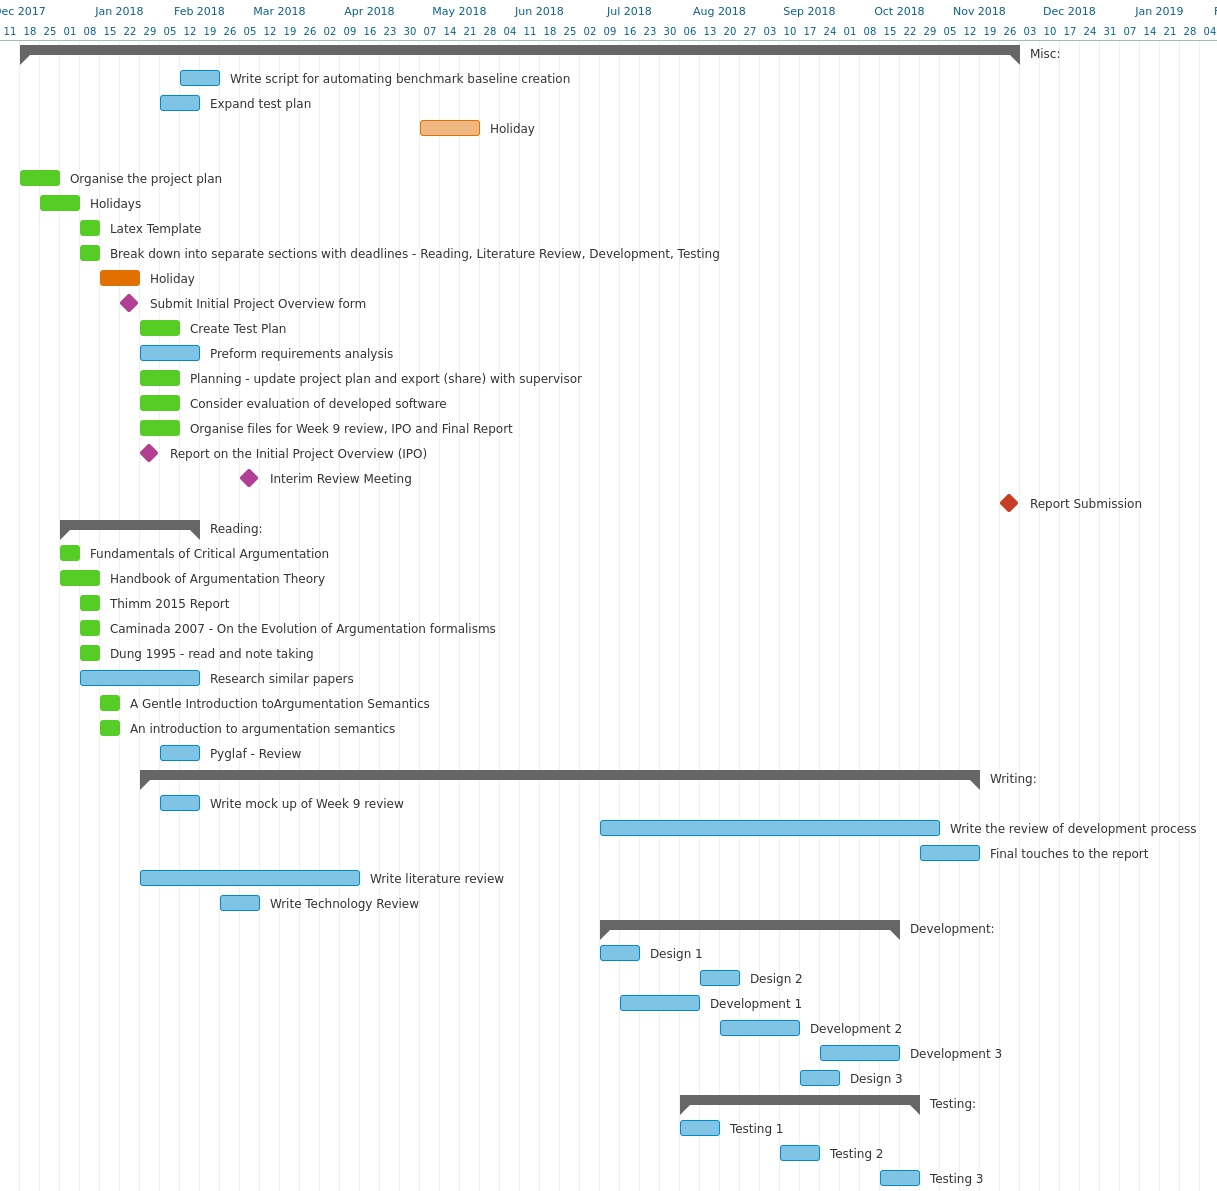
\includegraphics[width=\textwidth]{gantt1}
	\caption{Project Schedule}
	\label{fig:projectSchedule}
\end{figure}

\section{Meetings diaries}
\label{appendix:diaries}
\newpage
\includepdf{./diaries/20180116.pdf}
\includepdf{./diaries/20180123.pdf}
\includepdf{./diaries/20180130.pdf}
\includepdf{./diaries/20180206.pdf}
\includepdf{./diaries/20180213.pdf}
\includepdf{./diaries/20180220.pdf}
\includepdf{./diaries/20181008.pdf}

\section{ICCMA 2017 Submissions}
\label{appendix:ICCMASubmissions}
\begin{center}
\begin{longtable}{| p{.2\textwidth} | p{.8\textwidth} |}
\caption{ICCMA 2017 Submissions}
\label{table:ICCMA2017Submissions}\\

\hline \multicolumn{1}{|c|}{\textbf{Solver}} & \multicolumn{1}{c|}{\textbf{Author}}\\ \hline 
\endfirsthead


\multicolumn{2}{c}%
{{\bfseries \tablename\ \thetable{} -- continued from previous page}} \\
\hline \multicolumn{1}{|c|}{\textbf{Solver}} &
\multicolumn{1}{c|}{\textbf{Author}} \\ \hline 
\endhead

\hline \multicolumn{2}{|r|}{{Continued on next page}} \\ \hline
\endfoot

\hline \hline
\endlastfoot

argmat-clpb   & Fuan Pu (Tsinghua University, China), Guiming Luo (Tsinghua University, China), Yucheng Chen (Tsinghua University, China).                  \\ \midrule
argmat-dvisat & Fuan Pu (Tsinghua University, China), Guiming Luo (Tsinghua University, China), Ya Hang (Tsinghua University, China).                    \\ \hline
argmat-mpg & Fuan Pu (Tsinghua University, China), Guiming Luo (Tsinghua University, China), Ya Hang (Tsinghua University, China).                    \\ \hline
argmat-sat & Fuan Pu (Tsinghua University, China), Guiming Luo (Tsinghua University, China), Ya Hang (Tsinghua University, China).                    \\ \hline
ArgSemSAT  & Federico Cerutti (Cardiff University, UK), Mauro Vallati (University of Huddersfield, UK), Massimiliano Giacomin (University of Brescia, Italy), Tobia Zanetti (University of Brescia, Italy). \\ \hline
ArgTools   & Samer Nofal (German Jordanian University, Jordan), Katie Atkinson (University of Liverpool, UK), Paul E. Dunne (University of Liverpool, UK).              \\ \hline
ASPrMin    & Wolfgang Faber (University of Huddersfield, UK), Mauro Vallati (University of Huddersfield, UK), Federico Cerutti (Cardiff University, UK), Massimiliano Giacomin (University of Brescia, Italy). \\ \hline
cegartix   & Wolfgang Dvořák (TU Wien, Austria), Matti Järvisalo (University of Helsinki, Finland), Johannes P. Wallner (TU Wien, Austria).                 \\ \hline
Chimærarg  & Federico Cerutti (Cardiff University, UK), Mauro Vallati (University of Huddersfield, UK), Massimiliano Giacomin (University of Brescia, Italy).              \\ \hline
ConArg  & Stefano Bistarelli (Università di Perugia, Italy), Fabio Rossi (Università di Perugia, Italy), Francesco Santini (Università di Perugia, Italy).              \\ \hline
CoQuiAAS   & Jean-Marie Lagniez (Univ. Artois, France), Emmanuel Lonca (Univ. Artois, France), Jean-Guy Mailly (Univ. Paris Descartes, France).                \\ \hline
EqArgSolver   & Odinaldo Rodrigues (King's College London, UK).                                       \\ \hline
gg-sts  & Tomi Jahunen (Aalto University, Finland), Shahab Tasharrofi (Aalto University, Finland).                            \\ \hline
goDIAMOND  & Stefan Ellmauthaler (Leipzig University, Germany), Hannes Strass (Leipzig University, Germany).                           \\ \hline
heureka    & Nils Geilen (Universität Koblenz-Landau, Germany), Matthias Thimm (Universität Koblenz-Landau, Germany).                        \\ \hline
pyglaf  & Mario Alviano (University of Calabria, Italy).                                       
\end{longtable}
\end{center}


\section{Argumentation Framework Graph}
\label{appendix:aficcma}
\begin{figure}
	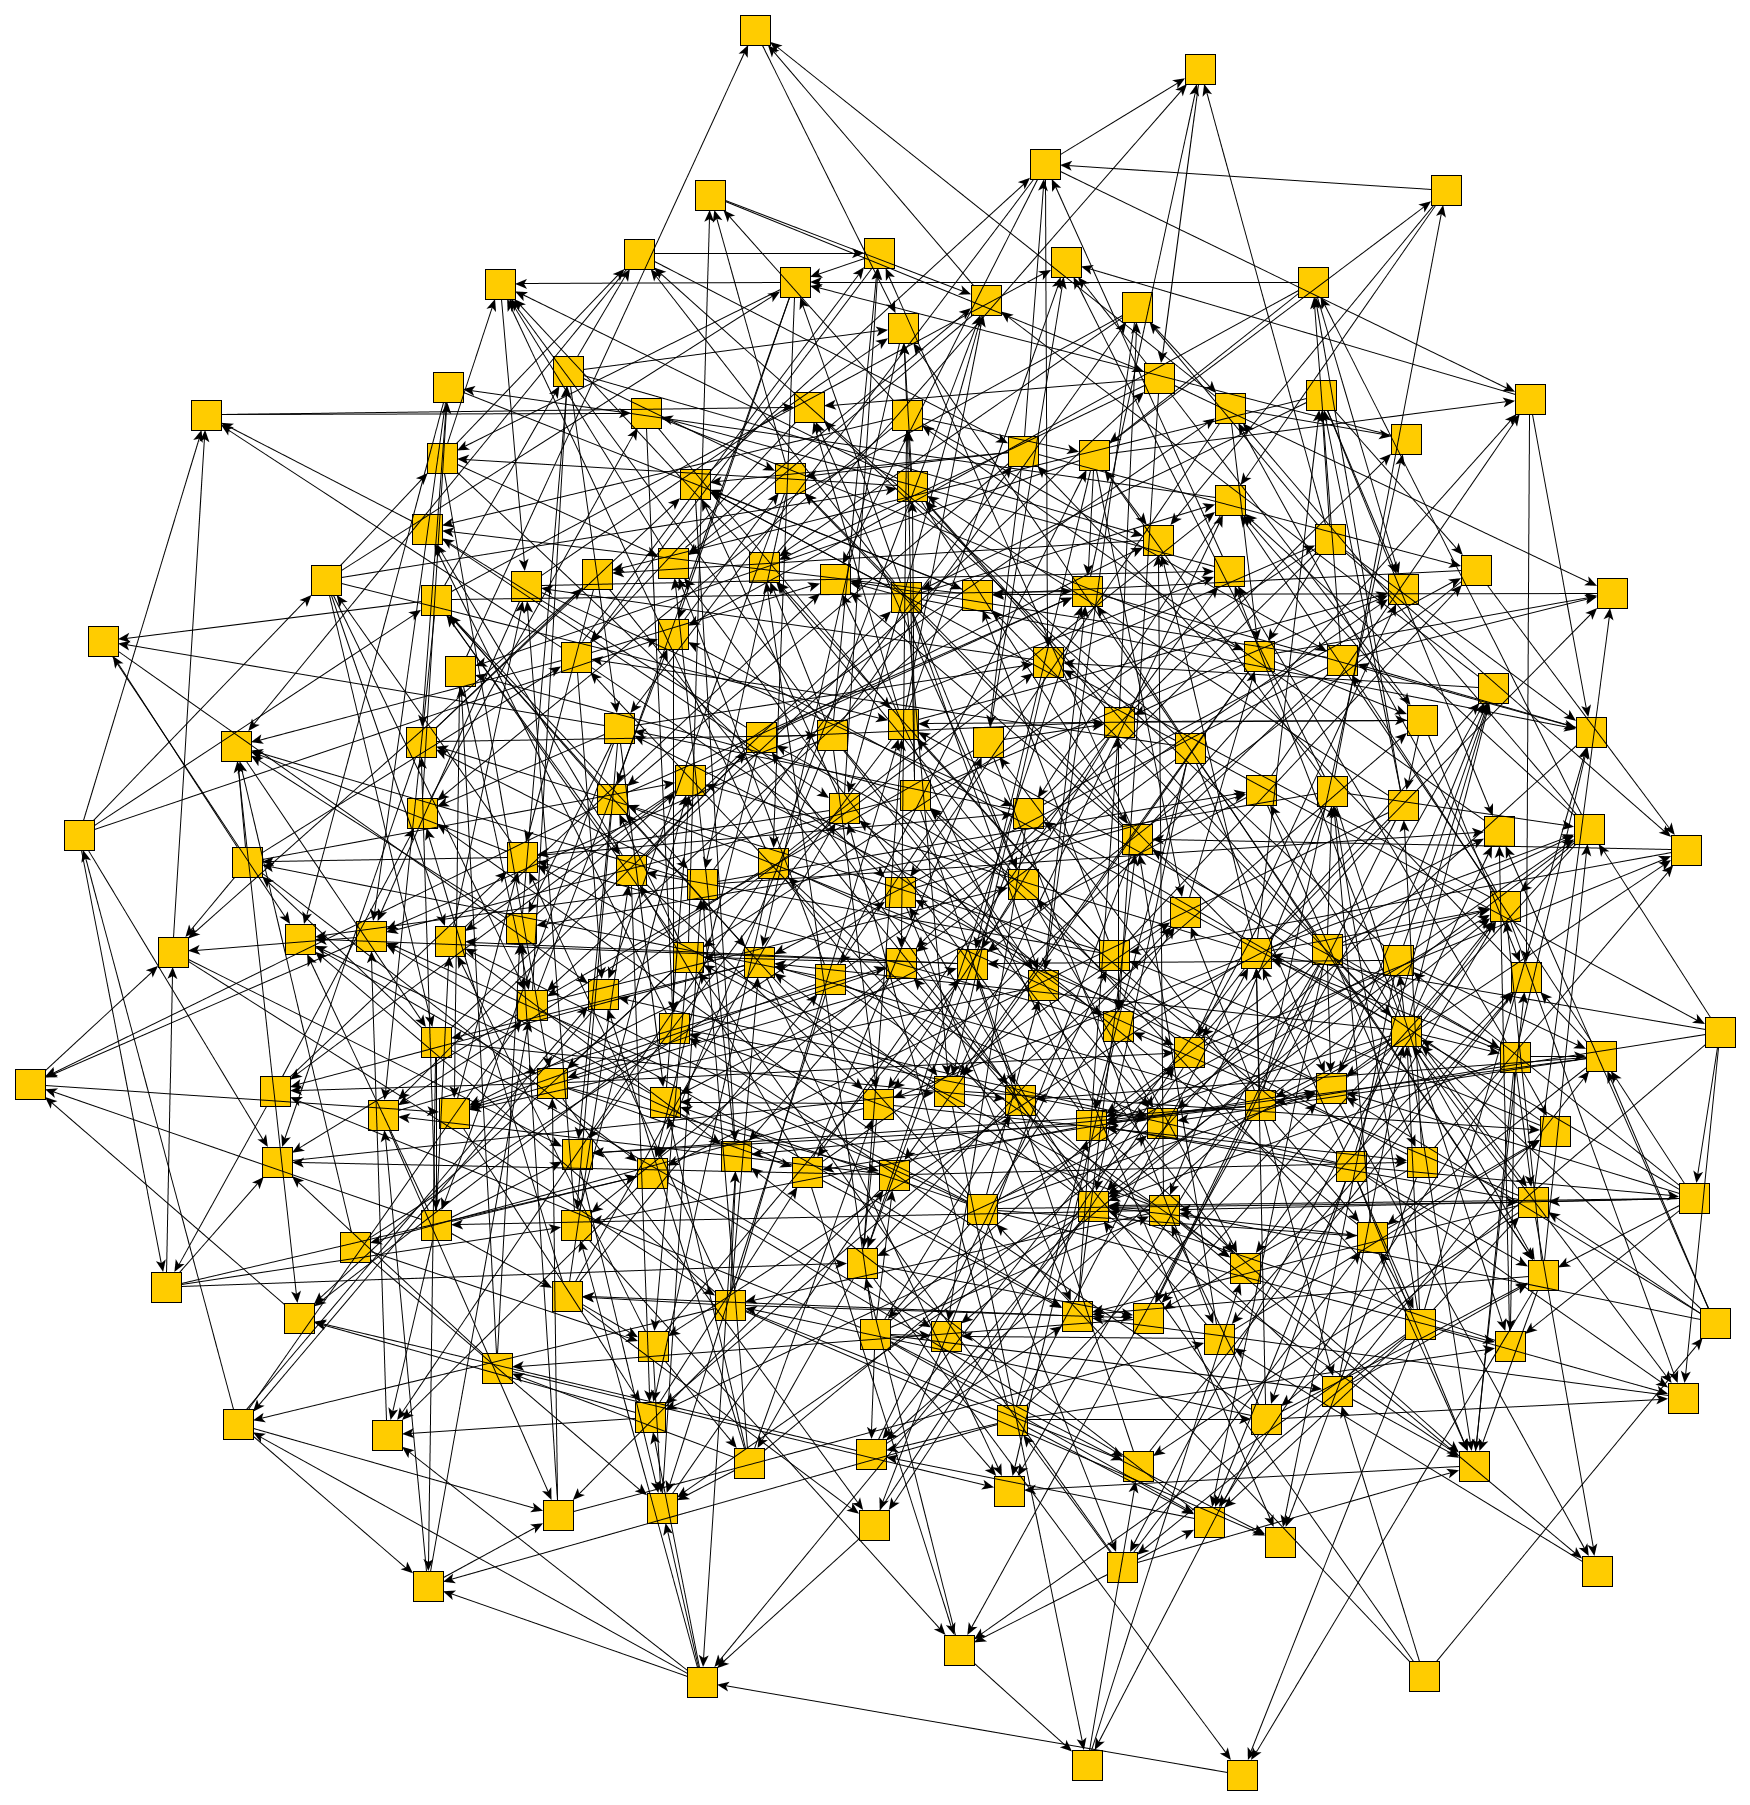
\includegraphics[width=0.9\textwidth]{AFICCMA}
	\caption{Example argumentation framework graph}
\end{figure}

%\begin{subappendices}
%\subsection{Example sub appendices}
...
%\end{subappendices}

%\section{Second Formal Review Output}
%Insert a copy of the project review form you were given at the end of the review by %the second marker

%\section{Diary Sheets (or other project management evidence)}
%Insert diary sheets here together with any project management plan you have

%\section{Appendix 4 and following}
%insert content here and for each of the other appendices, the title may be just on a page by itself, the pages of the appendices are not numbered, unless an included document such as a user manual or design document is itself pager numbered.
\end{appendices}

\end{document}
